\chapter{Datenextraktion} \label{Datenerhebung}
Nachdem ich die Forschungsfragen verfeinert habe, erhebe ich Merkmale und Zahlen aus den Videos, die der Beantwortung dieser dienen. Ich betrachte die Videos qualitativ und fertige Tabellen an, die Anzahlen der Personen mit gewissen Merkmalen und Verhaltensweisen, sowie Wechselzeiten enthalten. In diesem Kapitel erkläre ich die Methoden der Datenerhebung aus den Videos. Zudem gehe ich darauf ein, wie ich die Merkmale und Verhaltensweisen der Personen definiere.
\section{Methode der Extraktion: Tracking}\label{Tracking}
Bei der ersten Sichtung des Bildmaterials fiel mir ein Problem bei den Aufnahmen auf. Das frontale Filmen der Türen führt dazu, dass Fahrgäste, die nicht am Fahrgastwechsel der gefilmten Tür beteiligt sind, die Sicht auf diese versperren. Beispielhaft für dieses Problem ist die Abbildung \ref{fig:Problem bei Videos}.
\begin{figure}[H]
	\centering
		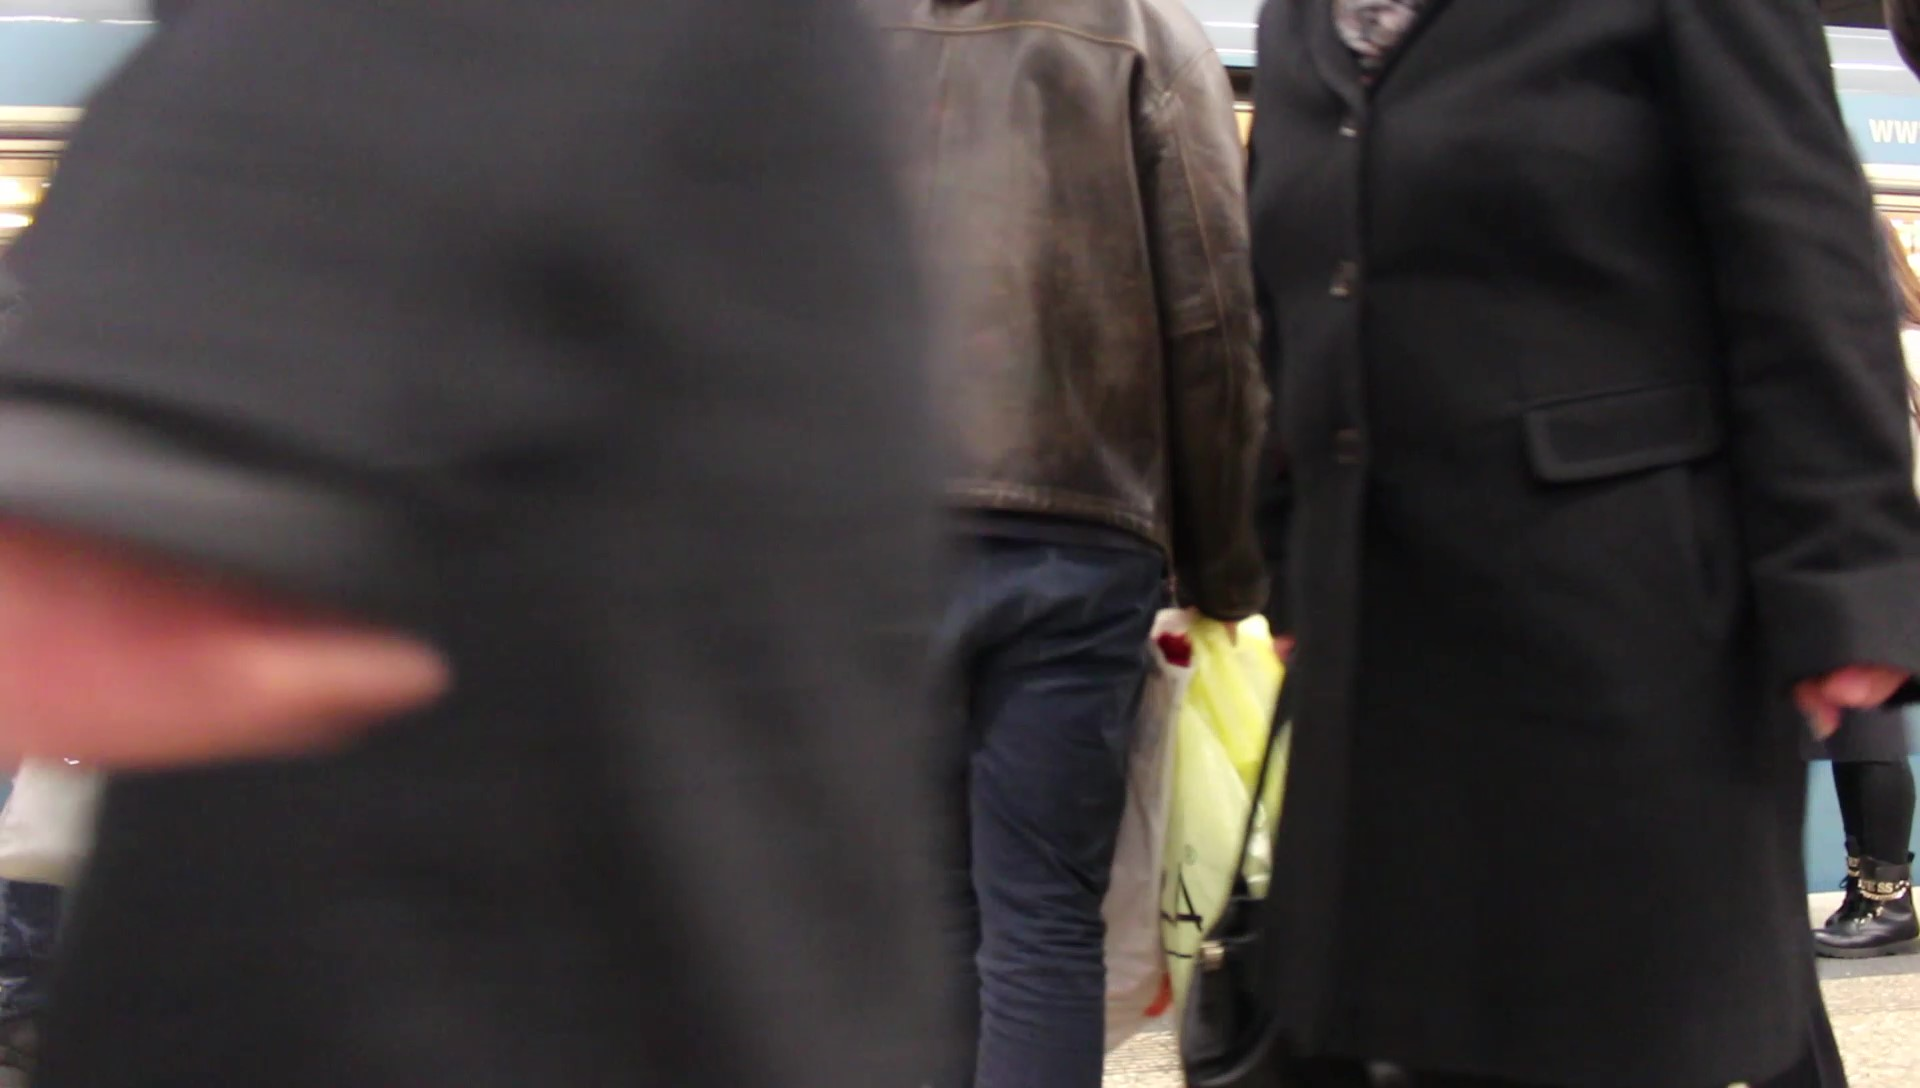
\includegraphics[width=0.65\textwidth]{pictures/data_extraction/tracking/problem.jpg}
	\caption{Beispiel für Probleme mit der Aufnahme: Personen, die durch das Bild laufen, versperren die Sicht auf den Fahrgastwechsel in der Tür.}
	\label{fig:Problem bei Videos}
\end{figure} 
Auf diesem Bild ist zu erkennen, dass die Sicht auf den Fahrgastwechsel in der gefilmten Tür versperrt ist.\\
Um eine genaue Zählung trotz dieses Problems zu ermöglichen, benutze ich die mir aus einem früheren Semester bekannte Software \textsf{Tracker}. Mit dieser Software kann ich die Videos Einzelbild für Einzelbild (eng.: "`Frame"') betrachten. Dadurch kann ich die Personen genauer zählen. Die Ansicht jedes Bildes ermöglicht mir zudem ein genaueres Messen der Fahrgastwechselzeiten. Die Einzelbilder, in denen der Fahrgastwechsel beginnt und endet kann ich so eindeutig identifizieren, wenn die Sicht auf die Tür frei ist. Die zugehörige Sekunde des Einzelbildes wird in der Software auf 3 Stellen genau angezeigt. Mit diesen genauen Zahlen kann ich dann genauer die Zeit messen, welche die Personen für den Wechsel benötigt haben. Jedoch nahm ich auch Filme auf, bei denen eine Person durch das Bild ging, wenn gerade die letzte Person einstieg. Dadurch kann ich auf diesen Videos das genaue Einzelbild des Fahrgastwechselendes nicht identifizieren. Für Filme, in denen dies geschah, schätzte ich den Moment, in dem das zweite Bein in den Wagen gesetzt wird. Im schlimmsten Falle wurde die Sicht auf den letzten Einsteiger 21 Frames lang versperrt. Ich schätzte jedoch, dass der Moment, in dem der zweite Fuß in den Wagon gesetzt wurde innerhalb von 10 der 21 Frames geschehen musste. Bevor die Person in das Bild gelaufen ist, war der Einsteiger noch etwas von der Tür entfernt und als die Person wieder aus dem Bild gegangen war, war die Person schon ein paar Schritte in den Zug gegangen. Deshalb konnten 6 Frames, nachdem die Person ins Bild gelaufen ist und 5 Frames bevor die Person wieder aus dem Bild ging, mit Sicherheit als nicht mögliche Zeitpunkte für das Fahrgastwechselende eliminiert werden. Ich schätze den Messfehler also auf \ca 10 Frames und damit, da ein Frame 0.033 Sekunden darstellt, auf 0.33 Sekunden. Deshalb wird ab nun die Fahrgastwechselzeit auf eine Stelle nach dem Komma gerundet.\\
Neben der Einzelbildansicht gibt es in diesem Tool die Möglichkeit, jeder Person eine sogenannte Punktmasse zuzuordnen und diese zu tracken. Dadurch wird verhindert, dass ein Fahrgast doppelt gezählt wird. Zudem kann ich dadurch das Verhalten und die Merkmale einer einzelnen Person über den gesamten Prozess besser beobachten. Der \textsf{Tracker} bietet zwei Möglichkeiten des Trackens. Zum einen kann eine Masse per Auto-Track verfolgt werden, zum anderen können die Personen per Hand in jedem Bild getrackt werden. Durch das Problem der versperrten Sicht war es nicht möglich das Auto-Tracking zu verwenden. Jede Person wurde von mir per Hand getrackt. In \figurename \ref{fig:tracking} kann das Tracking auf einem Bild eines der Videos betrachtet werden. Um den Vorgang des manuellen Trackings zu vereinfachen, tracke ich Aussteigende in unterschiedlichen Rottönen, Einsteigende in unterschiedlichen Blautönen. Platzmacher - auf diesem Bild nicht vorhanden - markierte ich in Grüntönen. \\
\begin{figure}[H]
	\centering
		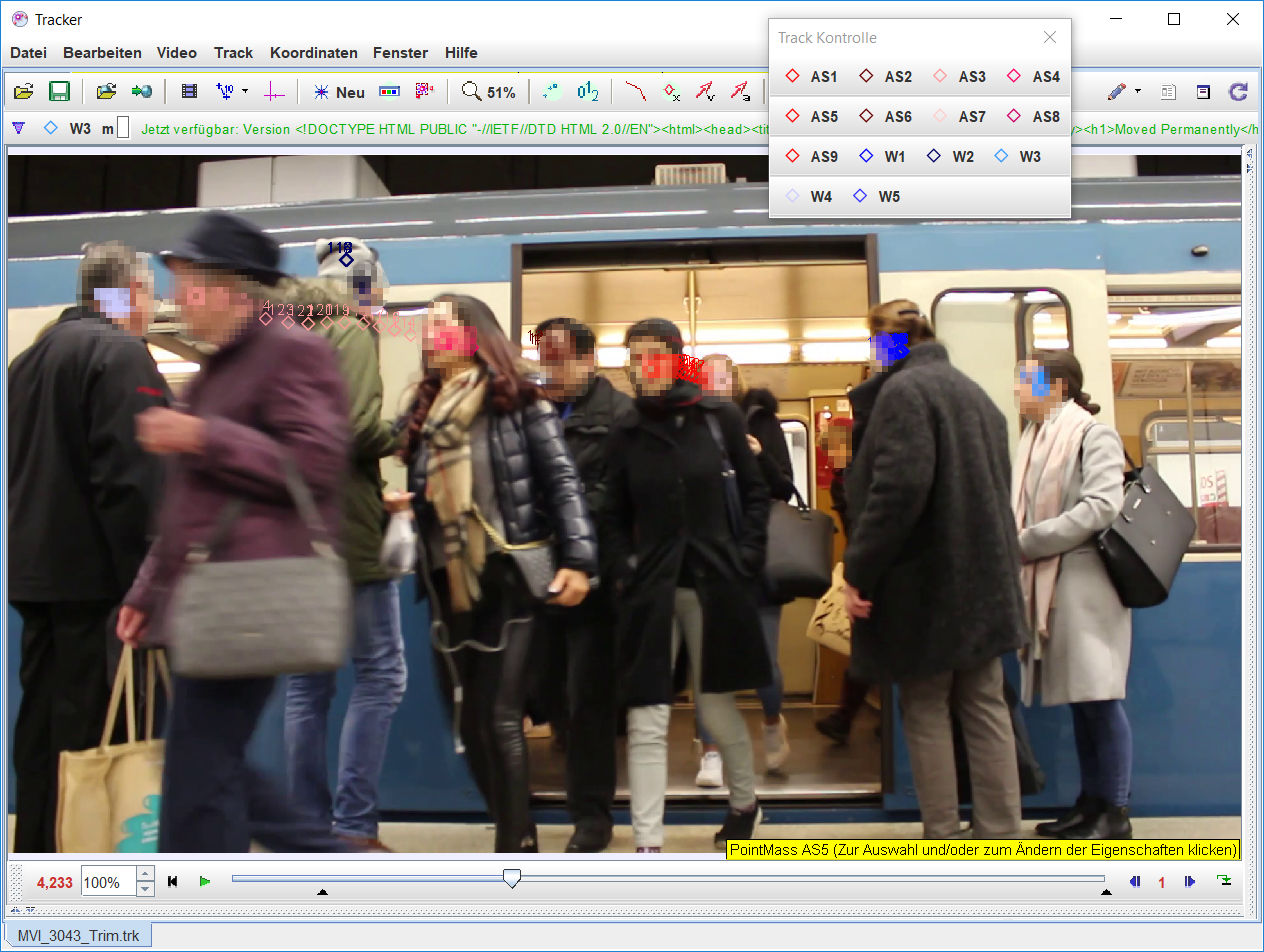
\includegraphics[width=0.7\textwidth]{pictures/data_extraction/tracking/trackExample.png}
	\caption{Screenshot der Software \textsf{Tracker}, mit Video und getrackten Personen. Aussteiger sind mit Rot, Einsteiger mit Blau gekennzeichnet.}
	\label{fig:tracking}
\end{figure}
\section{Tabellen} \label{Tabellen}
Für die unterschiedlichen Forschungsfragen erstellte ich Excel-Dateien, welche die Anzahlen von Personen und Zeiten enthalten, die ich mit dem Tracking-Tool aus den Videos gewonnen habe. Bei der Datenerhebung erstellte ich sieben CSV-Dateien in Excel. Dabei enthalten die einzelnen Dateien jeweils  Verhaltensweisen, Merkmale, Typen von Personen, Startzeiten der Aussteiger, Fahrgastwechselzeiten, sowie die erkannten Gruppen. Die Kopfzeilen der Tabellen sind in Englisch verfasst, um Probleme mit Umlauten bei der Weiterverarbeitung zu verhindern. \\
Jede Zeile der Tabellen enthält die jeweilige Anzahl der Merkmale und Verhaltensweisen und Zeiten für ein einzelnes Video. Diese trug ich nach der Sichtung des jeweiligen Videos in die entsprechenden Spalten ein. Zudem enthält die erste Spalte der Tabellen immer die Zahl des jeweiligen Videos (wie im Videonamen angegeben) um eine Zuordnung zu dem entsprechenden Film zu gewährleisten.
\subsection{Tabelle der Fahrgastwechselzeiten} \label{Zeiten Tabelle}
In der Tabelle der Fahrgastwechselzeiten hielt ich die Anzahlen der Kern-Einsteiger und Später-Einsteiger, sowie der Kern-Aussteiger und Später-Aussteiger fest. Daneben enthält die Datei die Anzahl der Platzmacher, die Kernwechselzeiten und die Fahrgastwechselzeiten.
Zudem diente mir diese Datei dazu, die Ankunftszeit der U-Bahnen und die Haltestelle, an der dieser Film gedreht wurde, festzuhalten. Im Anhang ist ein Ausschnitt der Tabelle, in \tablename \ref{tab:times}, eingefügt. \\
Die Verhaltensweisen später ein- oder aussteigen und die Begriffe Kern-Ein-, Kern-Aussteiger und Kernzeit sind wie folgt definiert:
\begin{longtable}{l p{10.5 cm}}
	\centering
			\textbf{Später-Einsteiger} & Als Später-Einsteiger werden Personen bezeichnet, die erst am Zug ankommen, wenn der Ausstiegsprozess beendet ist, und die ersten Wartenden schon mit dem Einsteigeprozess begonnen haben. Es werden jedoch nicht solche Personen beachtet, die erst einsteigen, wenn der Prozess schon einige Sekunden beendet war.\\
			 & \\
			\textbf{Kern-Einsteiger} & Anzahl der Personen die in den Zug einsteigen, ohne Zählung der Später-Einsteiger. (Anzahl Einsteiger - Anzahl Später-Einsteiger) \\
			 & \\
			 \textbf{Später-Aussteiger} & Als Später-Aussteiger werden Personen bezeichnet, die mit zeitlichem Abstand nach der Beendigung des Ausstiegsprozesses der übrigen Personen noch aus dem Zug aussteigen.\\
			 & \\
			\textbf{Kern-Aussteiger} & Anzahl der Personen die aus dem Zug aussteigen, ohne Zählung der Später-Aussteiger. (Anzahl Aussteiger - Anzahl Später-Aussteiger)\\
			 & \\
			 \textbf{Kernwechselzeit} & Die Kernwechselzeit beschreibt die Zeit, die Personen für den Fahrgastwechsel benötigen. Im Gegensatz zur Fahrgastwechselzeit werden hier keinerlei Ausreißer, in Form von Später-Ein- und Später-Aussteigern beachtet. Mit der Fahrgastwechselzeit kann also beschrieben werden, wie lange eine U-Bahn halten muss, während die Kernwechselzeit beschreibt wie lange eine gewisse Anzahl an Personen benötigt, um ein- und auszusteigen. \\
			 & \\
			 \textbf{Fahrgastwechselzeit} & Siehe \ref{Begriffe und Definitionen}.
\end{longtable}
Die Fahrgastwechselzeiten und Kernzeiten wurden dabei so mit Hilfe der im Tracking-Tool angegebenen Sekundenzahl gemessen. Dabei wird die Sekundenzahl des Einzelbildes in dem der erste Aussteiger einen Fuß auf den Bahnsteig setzt von der Sekundenzahl abgezogen, in der die letzte Person, die beachtet wurde, ihren zweiten Fuß in den Wagon setzt.

\subsection{Tabellen der Gruppen}
Für die Erfassung der Gruppengrößen erstellte ich drei separate Tabellen für die Prozesstypen Einsteiger, Aussteiger und Platzmacher. Diese enthalten in den Spalten jeweils die Anzahl der Gruppen mit der entsprechenden Gruppengröße für jedes Video. Ausschnitte der Tabellen können im Anhang in \tablename \ref{tab:groupsAS}, \tablename \ref{tab:groupsES} und \tablename \ref{tab:groupsPM} betrachtet werde. Gruppen wurden dabei durch das Verhalten ihrer Gruppenmitglieder identifiziert. Ich zähle Personen zu einer Gruppe, wenn sie mit anderen Personen reden oder auf andere Personen warten. Es ist möglich, dass so nicht jede Gruppe erkannt wird.

\subsection{Tabelle der Verhaltensweisen und Merkmale}
Die Tabelle der Verhaltensweisen und Merkmale enthält die jeweilige Anzahl der Personen, die bestimmte Verhaltensweisen und Merkmale in einem Video zeigen. Die Verhaltensweisen "`früher Einsteigen"' und "`im Weg Stehen"' werden in diese Tabelle eingetragen. Bei den Merkmalen handelt es sich um "`sperrig"', "`langsam"' und "`abgelenkt"'. Zudem enthält die Tabelle die Anzahl Einsteiger und Aussteiger sowie die Anzahl der Platzmacher. Auch die Fahrgastwechselzeit ist in dieser Tabelle enthalten. Die Ein- \bzw Aussteiger setzen sich aus der Summe der Kern-Ein- oder Kern-Aussteiger und der jeweiligen Später-Ein- oder Später-Aussteigern zusammen. Die genannten Merkmale und Verhaltensweisen werden wie folgt definiert:

\begin{longtable}{l p{10.5 cm}}
	\centering
			 \textbf{Im Weg Stehen} & Personen, die im Weg stehen, positionieren sich so vor der Tür, dass andere Personen, die ein- oder aussteigen einen Bogen um diese machen müssen.\\
			 & \\
			 \textbf{Früher Einsteigen}	& Einsteiger, die mit dem Prozess des Einsteigens beginnen, bevor die letzte Person den Zug verlassen hat. Diese Personen werden als Früher-Einsteiger bezeichnet.\\
			 & \\
			 \textbf{Sperrig} & Eine Person gilt als sperrig, wenn sie mehr Platz einnimmt als andere Personen. Es handelt sich um Personen, die ein großes  Gepäckstück mit sich tragen, einen Rollstuhl fahren oder schieben, einen Kinderwagen schieben oder einen Hund mit sich führen. \\
			 &\\
			 \textbf{Langsam} & Eine Person gilt als langsam, wenn die Beobachtende Person subjektiv den Eindruck hat, dass diese Person sich deutlich langsamer bewegt als andere.\\
			 &\\	
			 \textbf{Abgelenkt} & Abgelenkte Personen beschäftigen sich mit Gegenständen in ihrer Hand, die sie vom Prozess des Fahrgastwechsels ablenken. Auf den Videos gibt es Personen, die ihr Handy in der Hand halten und darauf schauen, sowie Personen die beim Aus- \bzw Einsteigen Zeitung lesen.\\
\end{longtable} 
\subsection{Tabelle der Typen} \label{Tabelle der Typen}
Auf den Filmen fallen mir folgende Typen von Verhaltensweisen auf: aggressiv, defensiv und normal. Die Tabelle der Typen für verschiedene Prozesstypen enthält in ihren Spalten für jeden der Prozesstypen die Anzahl, der Personen, die aggressives, defensives oder normales Verhalten zeigen. Zum genaueren Verständnis kann auch ein Ausschnitt der Tabelle in \tablename \ref{tab:Types} betrachtet werden.
\begin{longtable}{ l p {12 cm}}
	\centering
			 \textbf{Normal} 	& Normale Personen zeigen keine auffälligen Verhaltensweisen. Das heißt sie steigen aus oder ein, wenn genug Platz im Türbereich vorhanden ist. Es wird geschätzt, dass genügend Platz im Türbereich vorhanden ist, wenn im Türbereich das 1.2 Fache der Körperbreite der normalen Person frei ist. Diese Zahl wurde gewählt, da Normale den Türbereich betreten, wenn sie ohne Kontakt mit anderen Personen oder Hindernissen durch die Tür gehen können.\\ 
			 					& \\
			 \textbf{Defensiv} 	& Defensive Personen gehen eher langsamer. Sie gehen nur durch die Tür, wenn keine andere Person im Türbereich ist.\\
			 					& \\
			 \textbf{Aggressiv} & Aggressive Personen drängeln sich vor andere Personen und gehen dabei auch in deren Weg. Sie gehen bereits durch die Tür, wenn nur etwas Platz im Türbereich vorhanden ist. Es wurde geschätzt, dass aggressive Typen durch die Tür gehen, wenn das 0.8 Fache ihrer Körperbreite Platz in der Tür hat. Diese Zahl wurde gewählt, da Aggressive sich leicht seitlich drehen, wenn sie dadurch durch die Tür kommen. Sie gehen eher schneller als die anderen Typen oder laufen sogar.
\end{longtable}
Neben den allgemeinen Merkmalen für defensive, aggressive und normale Typen gibt es zudem noch Merkmale für die unterschiedlichen Prozesstypen, die nun definiert werden:
\begin{table}[H]
	\centering
		\begin{tabular}{ l p {3.5 cm} p {3.5 cm} p {3.5 cm} }
			\textbf{Prozesstyp}																	&\textbf{Normal} 																	&\textbf{Defensiv} 																	&\textbf{Aggressiv} \\
			\hline
			\textbf{Aussteiger}
			& Normale Aussteiger, die als erste aus dem Zug aussteigen, warten bis die Türen genügend weit geöffnet sind.
			& Defensive Aussteiger, die als erste aussteigen, warten bis die Türen des Zuges komplett geöffnet sind.
			& Aggressive Aussteiger, die als erste aussteigen, beginnen mit dem 				  Aussteigen, sobald die Türen etwas geöffnet sind.\\
			& & & \\
			\textbf{Einsteiger}
			& Normale Einsteiger beginnen mit dem Einsteigen, sobald genügend Platz im Türbereich vorhanden ist.
			& Defensive Einsteiger beginnen erst mit dem Einsteigen, nachdem die letzte Person den Zug verlassen hat, auch wenn genügend Platz zum Einsteigen vorhanden ist.
			& Aggressive Einsteiger beginnen mit dem Einsteigen sobald etwas Platz zum Einsteigen vorhanden ist. \\
			& & & \\
			\textbf{Platzmacher}
			& Normale Platzmacher stellen sich nach dem Aussteigen so weit nach vorne wie möglich, ohne im Weg zu stehen.
			& Defensive Platzmacher stellen sich nach dem Aussteigen hinter wartende Personen, auch wenn vorne Platz zum Hinstellen wäre.
			& Aggressive Platzmacher stellen sich vor die Wartenden, auch wenn sie dadurch im Weg stehen. \\
		\end{tabular}
\end{table}
Da es schwierig ist zu definieren, ab wann eine Tür etwas, genügend oder ganz geöffnet ist, nehme ich zudem die Startzeiten der Aussteiger in eine Tabelle, welche im Folgenden beschrieben wird.
\subsection{Tabelle der Startzeiten der Aussteiger}
Die Tabelle der Startzeiten der Aussteiger enthält den jeweiligen Typen des ersten Aussteigers (-1=defensiv, 0=normal, 1=aggressiv), die Sekunde im Video in der sich die Tür öffnet, die Sekunde in der  der Aussteiger den ersten Schritt macht, sowie die Zeit, die zwischen der Türöffnung und dem ersten Schritt des Aussteigers verstreicht. Auch für diese Tabelle wurde im Anhang, in \tablename \ref{tab:Startingtime}, ein Ausschnitt dieser eingefügt.